\documentclass[a4paper,10pt]{article}
\usepackage[utf8]{inputenc}
\usepackage[spanish]{babel}
\usepackage[affil-it]{authblk}
\usepackage{enumerate}
\usepackage{graphicx}
\usepackage{hyperref}
\usepackage{amsmath}
\usepackage{amssymb}
\usepackage{cancel}
\usepackage[usenames, dvipsnames]{color}
\usepackage{tikz}
\usepackage[labelfont=bf]{caption}
\usepackage{subcaption} %Multiple images
\usepackage{multicol} % Multiple columns
\usepackage{float}
\usepackage{cleveref}
 \usepackage{relsize} % bigger math symbols
\usepackage[margin=1.4in]{geometry}
\usepackage[titletoc,toc,title]{appendix}
\usepackage{enumitem}
\usepackage{etoolbox}
\usepackage{authblk} %multiple authors
\usetikzlibrary{calc}
\numberwithin{equation}{section}

% Circled words
\newcommand{\circled}[2][]{%
  \tikz[baseline=(char.base)]{%
    \node[shape = circle, draw, inner sep = 1pt]
    (char) {\phantom{\ifblank{#1}{#2}{#1}}};%
    \node at (char.center) {\makebox[0pt][c]{#2}};}}
\robustify{\circled}

%Appendices in spanish
\renewcommand{\appendixname}{Ap\'endices}
\renewcommand{\appendixtocname}{Ap\'endices}
\renewcommand{\appendixpagename}{Ap\'endices}

%Zero delimiter
\newcommand{\zerodel}{.\kern-\nulldelimiterspace}

%Columns separation
\setlength{\columnsep}{1cm}

%Indentation
\setlength{\parindent}{0ex}

%Multiple References

\crefrangelabelformat{equation}{(#3#1#4--#5\crefstripprefix{#1}{#2}#6)}

\usepackage{xparse}

%Boxes

\newcommand*{\boxcolor}{blue}
\makeatletter
\renewcommand{\boxed}[1]{\textcolor{\boxcolor}{%
\tikz[baseline={([yshift=-1ex]current bounding box.center)}] \node [rectangle, minimum width=1ex,rounded corners,draw] {\normalcolor\m@th$\displaystyle#1$};}}
 \makeatother

%Constantes
\newcommand{\euler}{\mathrm{e}}
\newcommand{\im}{i}

% Definición de las secciones y su numeración

\makeatletter
\def\@seccntformat#1{%
  \expandafter\ifx\csname c@#1\endcsname\c@section\else
  \csname the#1\endcsname\quad
  \fi}
\makeatother

%opening
\title{{\huge Reporte Preliminar} \\
\vspace{.2cm}
\large Laboratorio Avanzado - Detección de Rayos Cósmicos}

\author[1]{Favio Vázquez\footnote{\url{favio.vazquezp@gmail.com}}}
\author[2]{Susana Marín\footnote{\url{susyma3005@gmail.com}}}

\affil[1]{Instituto de Ciencias Nucleares,
Universidad Nacional Autónoma de México}
\affil[2]{Instituto de Química,
Universidad Nacional Autónoma de México}

\date{}

\begin{document}

\maketitle

\section*{Introducción}

Los rayos cósmicos fueron descubiertos por el físico Austríaco-Americano, Víctor
Hess. En 1912, Hess estableció que la ionización atmosférica aumenta con la
altitud, y concluyó que la “radiación” que la origina debía proceder del espacio
exterior lo que le valió el premio Nobel de Física del año 1936. En años posteriores
los rayos cósmicos fueron estudiados utilizando cámaras de destellos que permiten 
trazar la trayectoria y distinguir entre diferentes tipos de partículas cargadas que,
ya que éstas, en presencia de un campo magnético, son desviadas de una trayectoria
recta. Lo mismo ocurre con los rayos cósmicos durante su propagación hasta la 
tierra, y por lo tanto no son convenientes para las observaciones astronómicas. 

\vspace{.3cm}

Desde su descubrimiento se han hecho una gran cantidad de experimentos y grandes 
colaboraciones para estudiar las propiedades y la naturaleza de los rayos cósmicos. 
Hoy en día tenemos una gran idea de sus características y origen, la teoría 
más aceptada dice que los rayos cósmicos están compuestos por partículas cargadas 
estables, fotones y núcleos atómicos con tiempos de vida de al rededor de 
$10^6$ años o más. Técnicamente, podemos hablar que los rayos cósmicos primarios, 
están compuestos por partículas aceleradas desde fuentes astrofísicas y los secundarios 
son las partículas producidas en la interacción con las partículas de la atmósfera 
al llegar a la tierra. Sabemos que algunos provienen de adentro del sistema solar, 
otros de algún lugar de la galaxia y algunos pocos de afueras de nuestra galaxia. Pero 
el fenómeno físico completo aún no es entendido por completo, desde teorías muy plausibles 
y conservadoras, así como más radicales y exóticas se han propuesto para explicar 
el origen físico de los rayos cósmicos, y si lo que hoy en día sabemos es correcto, pero 
aún no hay un consenso completo sobre el tema. Es probable que con las nuevas mediciones 
de algunos grandes observatorios de rayos cósmicos comencemos a tener una mejor idea 
sobre la respuesta a estas preguntas, pero por ahora solo podemos mantenernos en espera 
y utilizar los resultados que se han obtenido hasta ahora.

\vspace{.3cm}

En este informe preliminar de laboratorio se muestran los resultados y breves análisis 
de los experimentos que hemos realizado. Dejamos para el segundo, y final informe una 
conclusión y análisis un poco más detallados de los resultados que se obtendrán y de 
los que ya se han obtenido. Hasta el momento hemos completado 2 experimentos, 
el primero era la medición del punto de operación del sistema que utilizaremos 
para el resto del laboratorio \eqref{ss:medicionoperacion}, en el cual se hicieron mediciones de muones atmosféricos 
\eqref{ss:componentemuonica} a distintos voltajes, para determinar en qué rango 
de operación se encuentra el plató en el cual el sistema es estable, así como 
el punto medio del rango que tomamos como el punto de operación del sistema. El otro experimento 
completo consistió en determinar la distribución angular de los muones \eqref{ss:medicionangulos} y utilizando 
el punto de operación obtenido anteriormente, se quería validar que el sistema 
cumplía con las expectativas teóricas para la distribución del flujo a distintos 
ángulos, así como el porcentaje de muones que llegan a distintos ángulos al 
laboratorio. La medición que falta por completar es la atenuación de muones con 
placas de plomo \eqref{ss:medicionplomo}, en la cual el plan es calcular cuánto afecta una cantidad dada 
de plomo, en atenuación, al flujo de muones que llegan al sistema.

\vspace{.3cm}

El reporte está dividido en 3 secciones, en la primera \eqref{s:marcoteorico} se comienza con una breve discusión 
teórica sobre rayos cósmicos, sus componentes, y su detección. En la segunda sección 
\eqref{s:metodologiaexperimental} se explica la metodología experimental seguida para la realización de cada uno de los 
experimentos y en la tercera sección \eqref{s:resultados} se muestran los resultados obtenidos y se 
hace un breve análisis de los mismos. Como ya se ha establecido al ser preliminar 
este reporte no se espera un tratamiento completo de cada experimento, y en el 
último que está en camino, nos muestra solamente el camino a seguir.

\section{Marco Teórico}
\label{s:marcoteorico}

\subsection{Rayos Cósmicos}

Los rayos cósmicos son partículas energéticas o fotones originadas en fuentes 
externas a la Tierra. Antes de entrar en la atmósfera de la Tierra, los rayos cósmicos 
primarios están compuestos en un $90\%$ por protones, un $9\%$ de partículas alfa y 
algunos núcleos pesados \cite{mok}. Los rayos cósmicos se extienden en un amplio 
rango de energía, hasta un máximo de alrededor de $10^{20}$ eV. Existen diferentes fuentes 
de rayos cósmicos y, de acuerdo a su origen, pueden ser categorizados en:

\begin{itemize}
 \item \textbf{Rayos cósmicos Solares}: Forman la componente de más baja energía 
 en el espectro de los rayos cósmicos y están asociados a la actividad solar. Son 
 partículas que tienen energía desde los pocos keV hasta algunos GeV o hasta 
 los $15-30$ GeV en los eventos de erupción solar poderosos.
 \item \textbf{Rayos cósmicos Galácticos}: Vienen de afuera del sistema solar pero 
 generalmente de adentro de la Galaxia, la Vía Láctea. Comúnmente están compuestos 
 de núcleos atómicos los cuales se han despojado de todos sus electrones circundantes 
 durante su paso a altas velocidades a través de la galaxia. Probablemente han sido 
 acelerados en los últimos pocos millones de años, y han viajado varias veces por 
 la galaxia, atrapados por el campo magnético galáctico. Han sido acelerados a 
 casi la velocidad de la luz, probablemente por los remanentes de supernovas. Mientras 
 viajan por el fino fas del espacio interestelar, algunos de ellos interactúan y 
 emiten rayos gamma, que es como sabemos que pasan por la Vía Láctea.
 \item \textbf{Rayos cósmicos Extra-Galácticos}: Están conformados por partículas 
 que provienen de afuera de nuestra galaxia. Sus energías comúnmente exceden los 
 $10^{15}$ eV. Se sabe muy poco de su procedencia, principalmente por la baja 
 estadística que tenemos sobre ellos, solamente $\sim 1$ de éstos llega a la 
 tierra por año por metro cuadrado. La mayoría de las estimaciones, basadas en 
 modelos teóricos y numéricos, predicen que están compuestos en su mayoría 
 de protones, pero algunos han teorizado que pueden estar compuestos por 
 partículas y entidades generadas en el universo muy temprano como del 
 decaimiento de partículas súper pesadas o defectos topológicos \cite{nagano}.
\end{itemize}

Los rayos cósmicos pueden ser usados como fuentes de partículas de altas energías 
para la producción de partículas fundamentales e, históricamente, han llevado 
al descubrimiento del positrón, el muón, el pión, el kaón, etc. Debido a que 
están cargados por naturaleza, los rayos cósmicos interactúan con los 
campos magnéticos y esto resulta en que sigan movimientos complicados. Esto 
induce muchos efectos diferentes sobre los rayos cósmicos por los campos magnéticos 
de la Tierra, el Sol y las galaxias, así como efectos de latitudes de la Tierra 
y de modulación por parte del Sol. Debido a estos y algunos otros efectos, 
la dirección de la información de la componente galáctica y extra-galáctica 
de los rayos cósmicos es perdida y por lo tanto estas componentes bombardean 
a la Tierra isotrópicamente. 

\vspace{.3cm}

Debajo se encuentra una imagen del espectro de los rayos cósmicos, donde podemos ver 
el gran rango de energías que cubren y que mientras aumenta la energía, el flujo 
de partículas que llegan a la tierra decrece exponencialmente.

\begin{figure}[H]
 \center 
 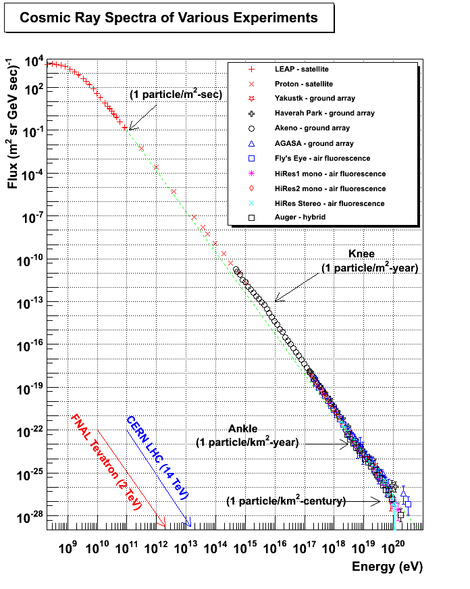
\includegraphics[scale=0.7]{fig1}
 \caption{Espectro energético de los rayos cósmicos.}
 \label{fig:fig1}
\end{figure}

Cuando los rayos cósmicos primarios entran a la atmósfera de la Tierra, interactúan 
con las moléculas de aire y producen muchos rayos cósmicos secundarios, principalmente 
protones, neutrones, piones y otras partículas, a través de reacciones nucleares. 
Debido a que muchas de estas partículas secundarias son todavía de muy alta energía, 
inician producciones subsecuentes de otras partículas en la forma de cascadas 
meso-nucleares y electromagnéticas. Estas cascadas nucleares-electromagnéticas complejas 
se conocen como lluvias extensas de aire o EAS\footnote{Extensive Air Shower.} en 
inglés. Fue notado por primera vez por Bruno Bossi que, en las mediciones de 
rayos cósmicos a nivel del mar, las cuentas de coincidencia de partículas 
medidas por los detectores de partículas separados en un plano horizontal 
excedían por mucho la coincidencia aleatoria. Pierre Auger y sus colaboradores 
hicieron luego algunas investigaciones más sistemáticas en este fenómeno y 
encontraron que los eventos de coincidencia ocurrían a separaciones horizontales 
tan grandes como 75 metros. La tasa de cuentas decrecía rápidamente cuando la 
distancia entre los contadores se aumentaba de los 10 cm a los 10 m, y luego 
la tasa se mantenía relativamente constante a distancia más grandes. Hubo mucho 
interés en el estudio de las EAS en los 1940's debido a que las energía de las 
partículas de la lluvia era mucha más alta que la producida en los aceleradores de 
partículas de la época. 

\begin{figure}[H]
 \center 
 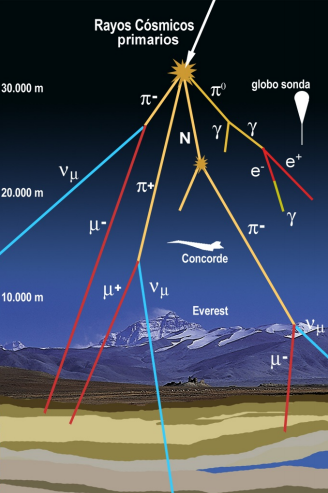
\includegraphics[scale=0.7]{fig2}
 \caption{Lluvias extensas de aire producidas por rayos cósmicos primarios, y la 
 producción subsecuente de rayos cósmicos secundarios.}
 \label{fig:fig2}
\end{figure}

\subsection{Componentes de la radiación cósmica}

Como ya se ha dicho, cuando un rayo cósmico llega a la atmósfera interactuará con 
una gran cantidad de átomos y moléculas. El proceso de interacción es bastante complejo, 
y tiene diferentes niveles. Debajo se encuentra un diagrama de las tres componentes 
que serán detalladas brevemente a continuación. 

\begin{figure}[H]
 \center 
 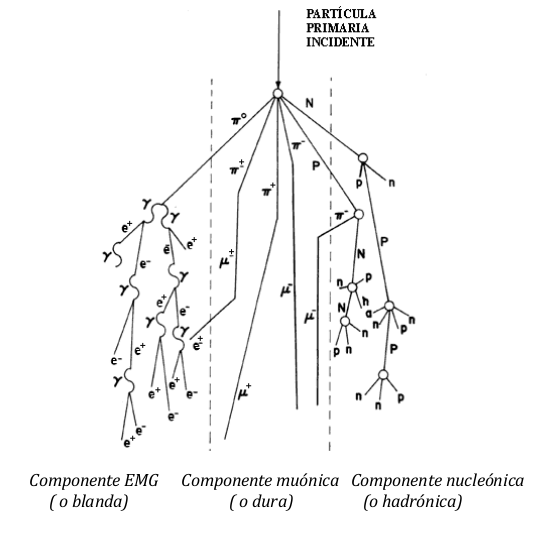
\includegraphics[scale=0.7]{fig3-1}
 \caption{Las distintas componentes de una radiación cósmica.}
 \label{fig:fig3}
\end{figure}

\subsubsection{Componente nucleónica}

Partiremos de un rayo cósmico primario, digamos un portón, imaginemos que llega a la 
atmósfera alta y choca con una molécula de oxígeno. Lo que esperaríamos que sucediera 
es que al golpearla, se produzca un efecto tipo juego de billar, en la cual las componentes 
de las partículas saldrían esparcidas por todo el aire. Luego de esto, desaparecerá 
el rayo cósmico primario y dará paso a un rayo cósmico secundario, que seguirá su 
camino llevando a cabo más reacciones energéticas posteriores. Los componentes 
nucleares iniciarán su camino descendente, interactuando con otros átomos 
y volviendo a producir nuevas interacciones nucleares. El proceso continua hasta 
que las nuevas partículas no tengan tanta energía para romper otros núcleos. Este 
proceso por lo general se detiene en la atmósfera, por lo que en la mayoría de los 
casos los rayos cósmicos primarios no llegan al suelo, pero pueden hacerlo ocasionalmente.

\subsubsection{Componente electromagnética}

La cascada se inicia cuando un núcleo primario choca con un núcleo atmosférico, 
produciendo una reacción nuclear en la que parte de la energía se transforma en 
materia, creándose nuevas partículas, sobre todo piones. Estos piones pueden 
ser positivos, neutros o negativos. Los piones neutros, que originarán una 
cascada electromagnética, decaen casi instantáneamente, convirtiéndose 
en dos fotones. Cada fotón produce un par $e^+$-$e^-$. Cada una de estas partículas 
avanza y emite un fotón que puede crear de nuevo un par $e^+$-$e^-$, y esto ocurre 
hasta que los fotones no tienen suficiente energía para crear nuevos pares. Esto 
está ilustrado en la parte izquierda de la figura \eqref{fig:fig3}.

\subsubsection{Componente muónica}
\label{ss:componentemuonica}

Los piones positivos y negativos creados, pueden interaccionar con otros núcleos, 
rompiéndolos, o decaer espontáneamente. Cuando un pión decae se convierte en 
un muón y en un neutrino muónico. El muón puede llegar al suelo o desintegrarse 
a su vez en un electrón, neutrino muónico y un neutrino electrónico. Esto puede 
verse en el centro de la imagen \eqref{fig:fig3}. Debido a que esta es la componente 
que más nos interesa debido a que fue la que medimos en el laboratorio, hablaremos 
un poco más de la misma.

\vspace{.3cm}

\textbf{Muones atmosféricos}

\vspace{.3cm}

La mayoría de los muones observados en la superficie de la Tierra, son producidos 
por rayos cósmicos primarios en la atmósfera superior. Son las más numerosas 
partículas energéticas que llegan al nivel del mar, con un flujo de aproximadamente 
1 muón por centímetro cuadrado por segundo. Esto se puede comparar con el flujo de
neutrinos solares de aproximadamente $5\times 10^6$ por centímetro cuadrado por segundo. 
Los muones pueden decaer por como:

\begin{equation}
\mu^- \rightarrow e^- + \overline{\nu_e} + \nu_\mu,
\end{equation}

\begin{equation}
 \mu^+ \rightarrow e^+ \nu_e + \overline{\nu_\mu}.
\end{equation}

La energía media de los muones que alcanzan el nivel del mar, es de aproximadamente
4 GeV. Los muones, siendo partículas, interactúan con la materia ionizándola. La 
pérdida de energía de los muones que pasan a través de la atmósfera, es proporcional
a la cantidad de materia que atraviesan. El medio se caracteriza generalmente por 
su densidad (g/cm$^3$), multiplicada por la distancia recorrida en centímetros. Esto
a veces se llama "longitud de interacción" y se mide en g/cm$^2$. La pérdida de 
energía de los muones es de aproximadamente 2 MeV por g/cm$^2$. La profundidad de la 
interacción con la atmósfera, es de unos 1000 cm$^2$, por lo que los muones pierden 
alrededor de 2 GeV al pasar por la atmósfera. Con una energía media de muones en la 
superficie del mar igual a 4 GeV, esto sugiere una energía original de muones en las
proximidades de 6 GeV.

\vspace{.3cm}

Se piensa que la mayoría de los muones se crean a una altura de unos 15.000 metros,
y viajan con otras partículas a la Tierra en lluvias cónicas, dentro de aproximadamente
1$^circ$ de la trayectoria de la partícula primaria que las crea. 

\subsection{Detección de rayos cósmicos}

Se han ideado diversos mecanismos de detección para rayos cósmicos. La mayoría de 
estos son muy complejos, algunos sencillos como el que utilizamos en el laboratorio. 
Y cada mecanismo está ideado para detectar algún tipo específico de rayo cósmico 
y sus componente. Debajo dos imágenes ilustran algunas técnicas de detección que 
se utilizan para estudiar los rayos cósmicos.


\begin{figure}[H]
 \center 
 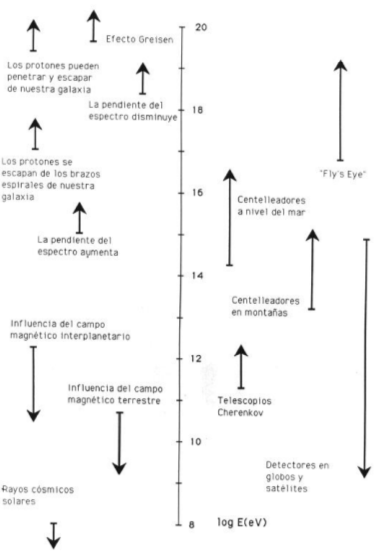
\includegraphics[scale=0.98]{fig4}
 \caption{Diferentes intensidades de rayos cósmicos y sus detectores.}
 \label{fig:fig4}
\end{figure}

\begin{figure}[H]
 \center 
 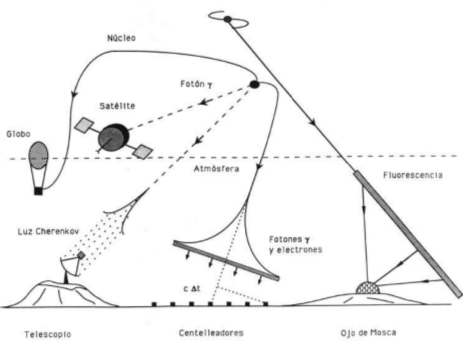
\includegraphics[scale=0.8]{fig5}
 \caption{Distintos detectores para rayos cósmicos.}
 \label{fig:fig5}
\end{figure}

Es muy extenso el material que existe y que se puede recopilar sobre detectores de 
rayos cósmicos pero sale del objetivo de este informe. Solo se hará un resumen de los 
detectores y aparatos que se usaron en el laboratorio para las distintas mediciones 
que se hicieron. En la subsección \eqref{ss:materialesutilizados} está una lista de 
todos los materiales utilizados para hacer las prácticas, ahora detallaremos brevemente
algunos de los equipos que usamos para hacer las mediciones.

\begin{itemize}
 \item \textbf{Centellador}: El centellador como su nombre lo indica centellea o exhibe 
 luminiscencia cuando por el pasa una partícula altamente energética. Este proceso
 se basan en la excitación atómica molecular, esto se produce cuando una partícula 
 muy  energética pero no cargada pasa a través del plástico centellador  y 
 este absorbe parte de la energía de la partícula incidente provocando una excitación
 a los electrones de la banda de valencia  hacia la banda de conducción, en cualquier 
 estado de activación cada electrón regresa a su estado base emitiendo un fotón de
 energía exactamente igual a la necesaria para pasar de su estado fundamental a su
 estado excitado la des-excitación causa la emisión de la luz en un proceso
 conocido como fluorescencia. Comúnmente están hechos de materiales orgánicos 
 o inorgánicos, los primeros se usan más para detecciones en el rango ultravioleta 
 y los inorgánicos para luz visible.
 \item \textbf{Guía de luz}: La guía de luz sirve para dirigir el camino de los fotones
 desde el centellador hasta el tubo fotomultiplicador. 
 \item \textbf{Tubo fotomultiplicador}: Los tubos fotomultiplicadores convierten 
 señales de luz provenientes de os centelladores que constan típicamente de no más 
 que unos cientos de fotones, en un pulso  de corriente utilizable sin añadir una 
 gran cantidad de ruido aleatorio a la señal.Los dos mayores componentes dentro del 
 tubo son una capa fotosensible, llamada  el \emph{fotocátodo}, acoplado a una 
 \emph{estructura multiplicadora de fotones}.  El fotocátodo sirve para convertir la
 mayor cantidad posible de fotones de luz  en electrones de baja energía. La sección
 de multiplicadora de electrones en un tubo fotomultiplicador provee una geometría
 de colección eficiente para los fotoelectrones, y sirve como un amplificador
 casi ideal para incrementar en altas cantidades su número. Luego de una 
 amplificación a través de la estructura multiplicadora, un pulso típico de
 centellador dará lugar a unos $10^7-10^{10}$ electrones \cite{knoll}, suficientes
 para servir de señal de carga para el evento original de centelleo. Esta carga
 es colectada convencionalmente en el ánodo o la etapa de salida de la estructura
 multiplicadora.
 \item \textbf{Discriminador}: Es un dispositivo que responde solamente a señales 
 de entrada con una altura de pulso mayor que cierto valor umbral. Si se satisface 
 este criterio, el discriminador responde emitiendo una señal lógica estándar, sino, 
 no hay ninguna respuesta. El principal uso para los discriminadores es bloquear 
 ruidos de baja amplitud desde los fotomultiplicadores u otros detectores \cite{leo}. Los 
 buenos pulsos son convertidos por una electrónica en pulsos lógicos, utilizando 
 un convertidor analógico-digital.
 \item \textbf{Compuerta AND}: Es una puerta lógica digital que implementa la
 conjunción lógica $-$ se comporta de acuerdo a la tabla de verdad mostrada a la 
 derecha. Ésta entregará una salida ALTA (1), dependiendo de los valores de las 
 entradas, siendo este caso, al recibir solo valores altos en ambas entradas. Si 
 alguna de estas entradas no son ALTAS, entonces se mostrará un valor de salida 
 BAJA (0). En otro sentido, la función de la compuerta AND efectivamente encuentra 
 el mínimo entre dos dígitos binarios, así como la función OR encuentra el máximo.
 Por lo tanto, la salida X solamente es ``1'' (1 lógico, nivel alto) cuando la entrada
 A como la entrada B están en ``1''. En otras palabras la salida X es igual a 1 cuando
 la entrada A y la entrada B son 1.
\end{itemize}


\section{Metodología Experimental}
\label{s:metodologiaexperimental}

\subsection{Materiales utilizados}
\label{ss:materialesutilizados}

A continuación se listan los materiales que fueron utilizados para las distintas mediciones:

\begin{itemize}
 \item Dos paletas centelladoras.
 \item Osciloscopio.
 \item Cables de 1, 3, 5, 10, 16 ns.
 \item Convertidores para cables.
 \item Fuente de alto voltaje.
 \item Placas de plomo.
 \item Flexómetro.
 \item Módulos de alto voltaje, temporización, discriminador y unidad lógica AND.
 \item Soporte de ángulo variable.
\end{itemize}


\subsection{Medición del punto de operación}
\label{ss:medicionoperacion}

Se utilizó un arreglo de centelladores, llamado arreglo de coincidencias, con el cual se desea medir el punto de operación del sistema, y el rango de operación del mismo, 
lo cual nos servirá para mediciones posteriores. A continuación se describen los 
pasos realizados para hacer la primera parte del diseño experimental.

\vspace{.3cm}

Pasos:

\begin{itemize}
 \item Se activan las paletas y se ponen para hacer coincidencia. Se conectan las paletas a la fuente de alto voltaje y 
 mediante el programa HyperTerminal se fija un voltaje inicial y se fue aumentando el voltaje lentamente. Las paletas 
 se colocan para hacer coincidencia una sobre la otra y se fijan a la mesa.
 \item Posteriormente se conectan las paletas al osciloscopio con cables de 10 ns  para comprobar la coincidencia, para esto se deben ajustar 
 las escalas de voltaje y temporal del osciloscopio. La escala temporal se fija al rededor de 80 ns y 
 el voltaje en 10 mV.
 \item Se conectan las paletas al discriminador con cables de la misma longitud, para evitar desfases en la señal.
 \item Se ajusta el voltaje del umbral (threshold) a 13 mV, y se revisa que exista coincidencia conectando cables de 
 16 ns al osciloscopio.
 \item Se conectan los canales correspondientes y se procede a tomar nota de las cuentas de partículas que llegan al sistema
 en coincidencia en un tiempo determinado, que fue de 5 minutos para cada voltaje.
 \item Estas mediciones se repiten para cada voltaje y así obtener una estadística del proceso de detección, se hace una tabla y 
 se grafican los valores.
\end{itemize}


\subsection{Medición de la distribución angular de los muones}
\label{ss:medicionangulos}

Esta medición se hizo para medir la distribución angular de los muones y determinar 
el porcentaje de los mismos que llegan desde todo lugar.

\vspace{.3cm}

Se utilizó el soporte de ángulo variable, se fijó una de las paletas en la parte 
inferior del soporte y la otra paleta en la parte superior, habiendo una distancia 
entre ellos dos de 7 cm. Se conectó el sistema y se comprobó la coincidencia
de la misma manera que en la sección anterior. Se fue girando el dispositivo cada 
10 grados, partiendo de $0^\circ$ hasta $90^\circ$, y se anotó el número de cuentas 
de muones para cada ángulo en un tiempo de 5 minutos por medición, en la sección
de resultados se encuentran estos datos tabulados y graficados.

\subsection{Medición de la Atenuación de Muones mediante el uso de plomo}
\label{ss:medicionplomo}

En esta sección el objetivo principal es cuantificar la atenuación de muones en 
función de la densidad del material utilizado para atenuar, en este caso el plomo, 
y la distancia entre las paletas. 

\vspace{.3cm}

Se conectaron los cables de la misma manera que en
las secciones anteriores, se fija un voltaje de 740 V consistente con el punto de 
operación, y antes de comenzar las 
mediciones se comprobó que hubiera coincidencia, y se hicieron mediciones para saber
si el aparato experimental se encontraba calibrado. Se acomodaron los bloques de plomo 
de tal manera que se forma una estructura que tenga un lado abierto y la parte 
superior descubierta, por el cual se introdujo una de las paletas. Para tener un 
punto de referencia, se colocó un bloque de hule espuma sobre la estructura de plomo,
y la segunda paleta sobre este bloque, cuidando que la segunda se encontrara 
exactamente sobre la primera, de modo que se tenga coincidencia, habiendo una 
distancia de 21 cm entre las paletas. Se utilizó hule espuma, debido a su baja 
densidad y gracias a esta propiedad se puede tomar como referencia. Se anotó el 
número de cuentas cada cinco minutos. Posteriormente se sustituyó el bloque de hule
espuma, por un bloque de plomo, se acomodaron las paletas de la misma manera a 21 cm
y se realizó la misma medición. El plan siguiente es ir aumentando el número de bloques de tal
manera que la atenuación aumente hasta dejar de tener cuentas en un tiempo dado. 
Se harán las mediciones primero con hule espuma para tener una referencia y
posteriormente se sustituyen con plomo.

\section{Resultados}
\label{s:resultados}

Todos los errores reportados en las siguientes tablas fueron calculados con la desviación 
estándar, cuya ecuación es 

\begin{equation}
 \sigma = \sqrt{\frac{1}{N}\sum_{i=1}^N (x_i - \mu)^2},
\end{equation}

donde $N$ es la cantidad de datos, $\mu = \frac{1}{2} \sum_{i=1}^N x_i$ es la 
media de los datos y $x_i$ es cada dato puntual. Esta fue calculada con la 
función \href{http://distributionsjl.readthedocs.org/en/latest/univariate.html?highlight=std\#std}{$\texttt{std}$} 
del paquete $\texttt{Distributions}$ de Julia.


\subsection{Medición del punto de operación}

Se realizaron tres mediciones debido a que los errores en las primeras dos fueron muy altos, 
ya que habían problemas con el cableado, y mucho ruido desde la fuente de la alto voltaje,
y en el sistema en general. La medición que fue tomada en cuenta para calcular el 
punto y rango de operación fue la tercera, que consistió en 5 mediciones para cada voltaje 
partiendo de 650 V a 850 V, subiendo de el voltaje de 20 en 20. 


\begin{table}[H]
\centering
\caption{Mediciones a distintos voltajes para el flujo de muones}
\resizebox{\linewidth}{!}{%
\begin{tabular}{|l|l|l|l|l|l|l|l|}
\hline
Voltaje & Medición 1 & Medición 2 & Medición 3 & Medición 4 & Medición 5 & Promedio & Error \\ \hline
650 & 90 & 89 & 91 & 104 & 90 & 92.8 & 6.3 \\ \hline
670 & 133 & 113 & 130 & 135 & 123 & 126.8 & 8.9 \\ \hline
690 & 135 & 138 & 147 & 146 & 133 & 139.8 & 6.3 \\ \hline
710 & 131 & 131 & 159 & 152 & 142 & 143.0 & 12.5 \\ \hline
730 & 153 & 142 & 157 & 153 & 170 & 155.0 & 10.0 \\ \hline
750 & 148 & 139 & 138 & 146 & 149 & 144.0 & 5.1 \\ \hline
770 & 139 & 146 & 168 & 159 & 159 & 154.2 & 11.5 \\ \hline
790 & 143 & 148 & 168 & 171 & 165 & 159.0 & 12.6 \\ \hline
810 & 144 & 140 & 162 & 177 & 178 & 160.2 & 17.8 \\ \hline
830 & 178 & 166 & 192 & 173 & 204 & 182.6 & 15.2 \\ \hline
850 & 180 & 195 & 197 & 199 & 193 & 192.8 & 7.4 \\ \hline
\end{tabular}}
\end{table}

\begin{figure}[H]
 \center 
 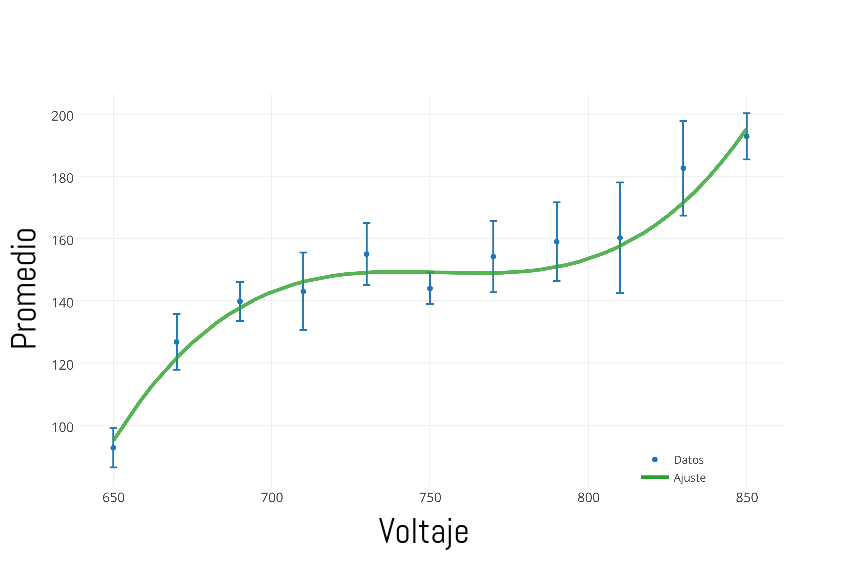
\includegraphics[scale=0.38]{atenuacionMuones1}
 \caption{Distribución angular de muones y curva de mejor ajuste.}
\end{figure}

De la anterior gráfica observamos que el rango de operación está entre 690 V y 770 V,
y por lo tanto tomamos el punto de operación como 740 V. 

\subsection{Medición de la distribución angular de los muones}

Debajo se muestra la tabla de datos registrados para la medición de distribución 
angular de los muones,

\begin{table}[H]
\centering
\caption{Mediciones a distintos ángulos para el flujo de muones}
\begin{tabular}{|l|l|l|l|l|l|}
\hline
Ángulo & Medición 1 & Medición 2 & Medición 3 & Promedio & Error \\ \hline
0      & 48        & 42        & 42        & 44.0     & 3.4   \\ \hline
10     & 39        & 31        & 42        & 37.3     & 5.6   \\ \hline
20     & 31        & 37        & 38        & 35.3     & 3.7   \\ \hline
30     & 23        & 30        & 34        & 29.0     & 5.5   \\ \hline
40     & 27        & 23        & 24        & 24.6     & 2.0   \\ \hline
50     & 24        & 21        & 23        & 22.6     & 1.5   \\ \hline
60     & 16        & 14        & 14        & 14.6     & 1.1   \\ \hline
70     & 11        & 11        & 7         & 9.6      & 2.3   \\ \hline
80     & 4         & 6         & 3         & 4.3      & 1.5   \\ \hline
90     & 5         & 4         & 4         & 4.3      & 0.5   \\ \hline
\end{tabular}
\end{table}

Notamos una caída conforme nos acercamos a los 90$^\circ$  pues al estar las paletas en 
los 0$^\circ$ (en el zenit) el numero de cuentas es mayor ya que los muones procedentes 
de los rayos cósmicos caen directamente sobre las  paletas y conforme no vamos moviendo  
a los 90$^\circ$  el número de cuentas disminuye  ya que las partículas
interaccionan con otras(presentes en el ambiente) antes de  llegar a las paletas y 
así de esta manera las partículas que pasan a través de las paletas  son mucho menor. 
Debajo se encuentra graficada esta tabla y el mejor ajuste que será discutido a continuación,

\begin{figure}[H]
 \center 
 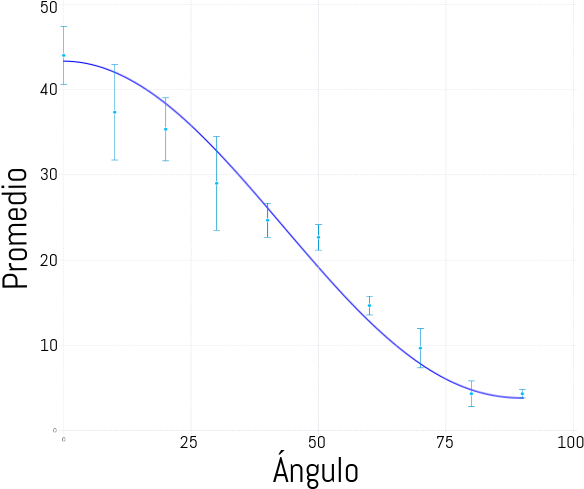
\includegraphics[scale=0.5]{ajusteAngulos}
 \caption{Distribución angular de muones y curva de mejor ajuste.}
 \label{fig:ajusteAngulos}
\end{figure}

Junto con los puntos y las barras de error se encuentra la línea de mejor ajuste. Crookes 
y Rastin en 1972 \cite{crookes} determinaron que la distribución del flujo es proporcional 
a $\cos^{2.16}{\theta}$, donde $\theta$ es el ángulo medido con respecto al zenit. La 
ecuación completa para el flujo a diferentes ángulos es 

\begin{equation}
 F(\theta) = F_v\cos^{2.16}{\theta},
\end{equation}

donde $F_v$ es el flujo vertical. Este parámetro se ajusta dependiendo del ángulo 
sólido sobre el cual se hacen las mediciones y la ventana de tiempo en la que se 
hace la medición. En nuestro caso el mejor ajuste, que es la línea azul sólida 
en la figura \eqref{fig:ajusteAngulos} fue de 

\begin{equation}
  F(\theta) = 40\cos^{2.16}{\theta} + 4 ,
\end{equation}

con lo cual hemos demostrado experimentalmente lo predicho por la teoría, claro 
con ciertos errores visibles en las barras de error entre los 10 y 30 grados.



\subsection{Medición de la Atenuación de Muones mediante el uso de plomo}

En esta sección no tenemos muchos resultados que mostrar debido a que solo se ha 
comenzado a hacer las mediciones. Solo se ha hecho una medición en el vacío y 
una con plomo y debajo se muestran estos puntos.

\vspace{.3cm}

Consideramos que el hule espuma que utilizamos en las primeras mediciones sin atenuación  como  un vacío debido a que su densidad es muy baja. El volumen de la 
pieza que usamos era de 1125 cm$^3$ y su masa es de $25.7414$ g, por lo tanto 
su densidad es $\rho = 0.022$ g/cm$^3$. Claramente no nos referimos a un vacío 
físico, sino que como su densidad es muy parecida al aire, y comparada con la 
densidad del plomo que es de $11.34$ g/cm$^3$, puede considerarse como un vacío.

\begin{table}[H]
\centering
\caption{Medición en el vacío.}
\begin{tabular}{|c|c|c|c|c|c|c|c|}
\hline 
Distancia & \#1 & \#2 & \#3 & \#4 & \#5 & Promedio & Error \\ 
\hline 
21 cm & 14 & 12 & 10 & 13 & 10 & 11.8 &  1.78 \\ 
\hline 
\end{tabular}
\end{table}

\begin{table}[H]
\centering
\caption{Medición con plomo.}
\begin{tabular}{|c|c|c|c|c|c|c|c|c|c|}
\hline 
Distancia & \#1 & \#2 & \#3 & \#4 & \#5 & \#6 & \#7 & Promedio & Error \\ 
\hline 
21 cm & 6 & 8 & 9 & 6 & 8 & 9 & 9 & 7.8 & 1.3 \\ 
\hline 
\end{tabular}
\end{table}

Claramente esperamos ver más atenuación mientras más plomo se le agregue al arreglo, 
y es la medición que falta por realizar.

\begin{thebibliography}{10}
\bibitem{mok}
H. Mok, \emph{Cosmic Rays: Climate, Weather and Applications}, Nova Publishers, 
2012.
\bibitem{nagano}
M. Nagano y A. Watson, \emph{Observations and implications of the ultrahigh-energy 
cosmic rays}, Reviews of Modern Physics \textbf{72}, pp. 689-732.
\bibitem{knoll}
G. Knoll, \emph{Radiation Detection adn Measurement}, 4ta edición, John Wiley \& Sons,
2010.
\bibitem{leo}
W. Leo, \emph{Techniques for nuclear and particle physics experiments: a how to 
approach}, 2da edición, Springer-Verlang, 1987.
\bibitem{crookes}
J. Crookes y B. Rastin, \emph{An Investigation of the Absolute Intensity of Muons at Sea Level}, 
Nucl Phys B \textbf{39}, p. 493, 1972.
\end{thebibliography}


\end{document}